\documentclass[tikz,border=5mm]{standalone}
\usepackage{tikz}
\usetikzlibrary{calc}

\begin{document}
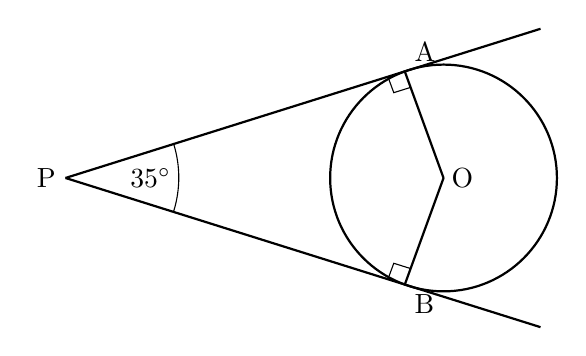
\begin{tikzpicture}[scale=1.2]

% Parameters
\pgfmathsetmacro{\radius}{1.2}

% Points
\coordinate (O) at (3,0);
\coordinate (P) at (-1,0);

% Tangent points A and B on circle
\coordinate (A) at ($(O)+(110:\radius)$);
\coordinate (B) at ($(O)+(250:\radius)$);

% Draw circle
\draw[thick] (O) circle (\radius);

% Draw tangent lines from P through A and B, extended beyond
\draw[thick] (P) -- ($(A)!-0.4!(P)$);
\draw[thick] (P) -- ($(B)!-0.4!(P)$);
\draw[thick] (O) -- (A);
\draw[thick] (O) -- (B);

% Right angle mark at A
\coordinate (A1) at ($(A)!0.15!(O)$);
\coordinate (A2) at ($(A)!0.05!(P)$);
\coordinate (A3) at ($(A1)+(A2)-(A)$);
\draw (A1) -- (A3) -- (A2);

% Right angle mark at B
\coordinate (B1) at ($(B)!0.15!(O)$);
\coordinate (B2) at ($(B)!0.05!(P)$);
\coordinate (B3) at ($(B1)+(B2)-(B)$);
\draw (B1) -- (B3) -- (B2);

% Calculate angle for arc at P
\pgfmathsetmacro{\anglePA}{atan2(1.5*sin(145), 3+1.5*cos(145)-(-1))}
\pgfmathsetmacro{\anglePB}{atan2(1.5*sin(215), 3+1.5*cos(215)-(-1))}

% Angle arc at P
\draw ($(P)!12mm!(A)$) arc (\anglePA:\anglePB:12mm);

% Labels
\node[left] at (P) {P};
\node[above right] at (A) {A};
\node[below right] at (B) {B};
\node at ($(O)+(0.2,0)$) {O};
\node at ($(P)+(0.9,0)$) {$35^{\circ}$};

\end{tikzpicture}
\end{document}